\section{Wprowadzenie}

Sytuacje nietypowe są to takie sytuacje,
które odbiegają od normalnie obserwowanych zachowań.
Może to być awaria, przeciążenie systemów,
trwający atak komputerowy z zewnątrz czy próba oszustwa.

Wykrywanie zmian (\textit{changepoint detection}) jest procesem
wykrycia w strumieniu czasowym wzorców (zmian zachowań, charakterystyk) nie pasujących do wcześniej zaobserwowanych.
Zmiany mogą mieć wiele różnych form.
Strumień danych może w pewnym momencie charakteryzować się rozkładem Gaussa,
aby nagle zmienić się na rozkład Poissona.
Przykładem takiej formy jest zachowanie czujnika światła (rys. \ref{fig:SignalDevice}).
W ciągu dnia, gdy jest słoneczna pogoda na chwilowe wartości może mieć wpływ zachmurzenie, przechodzące osoby, itp.
W nocy wachania są mniejsze.
\begin{figure}[htbp]
\centering
	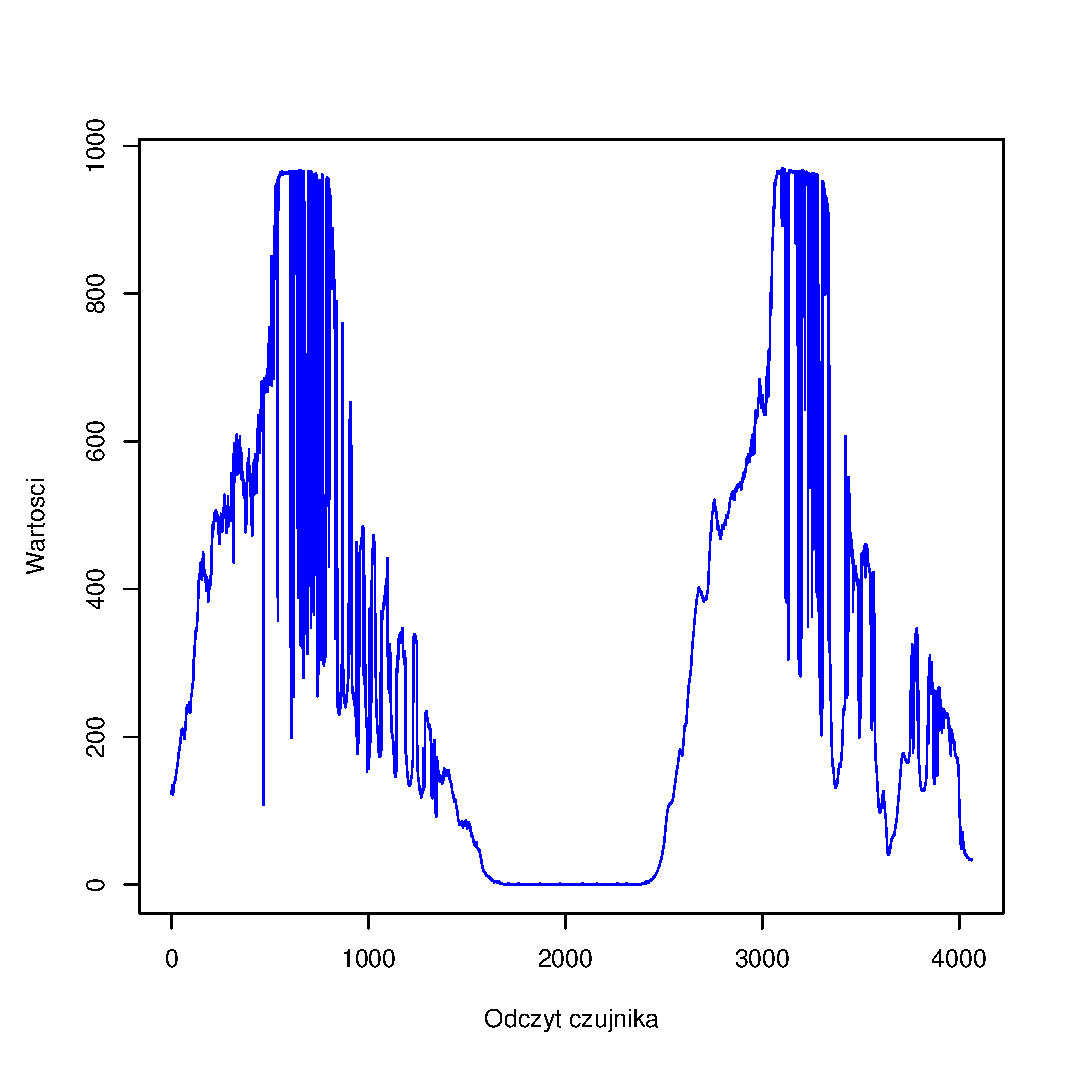
\includegraphics[width=0.6\textwidth]{img/ch-2-device}
	\caption{Wartości czujnika światła -- wachania w rytmie dzień/noc}
  \label{fig:SignalDevice}
\end{figure}
Inną formą może być zmiana parametrów rozkładu.
Przykładowo w strumieniu opisanym rozkładem Gaussa
w pewnym momencie czasu mogło nastąpić przesunięcie średniej (rys. \ref{fig:SignalData}).
\begin{figure}[htbp]
\centering
	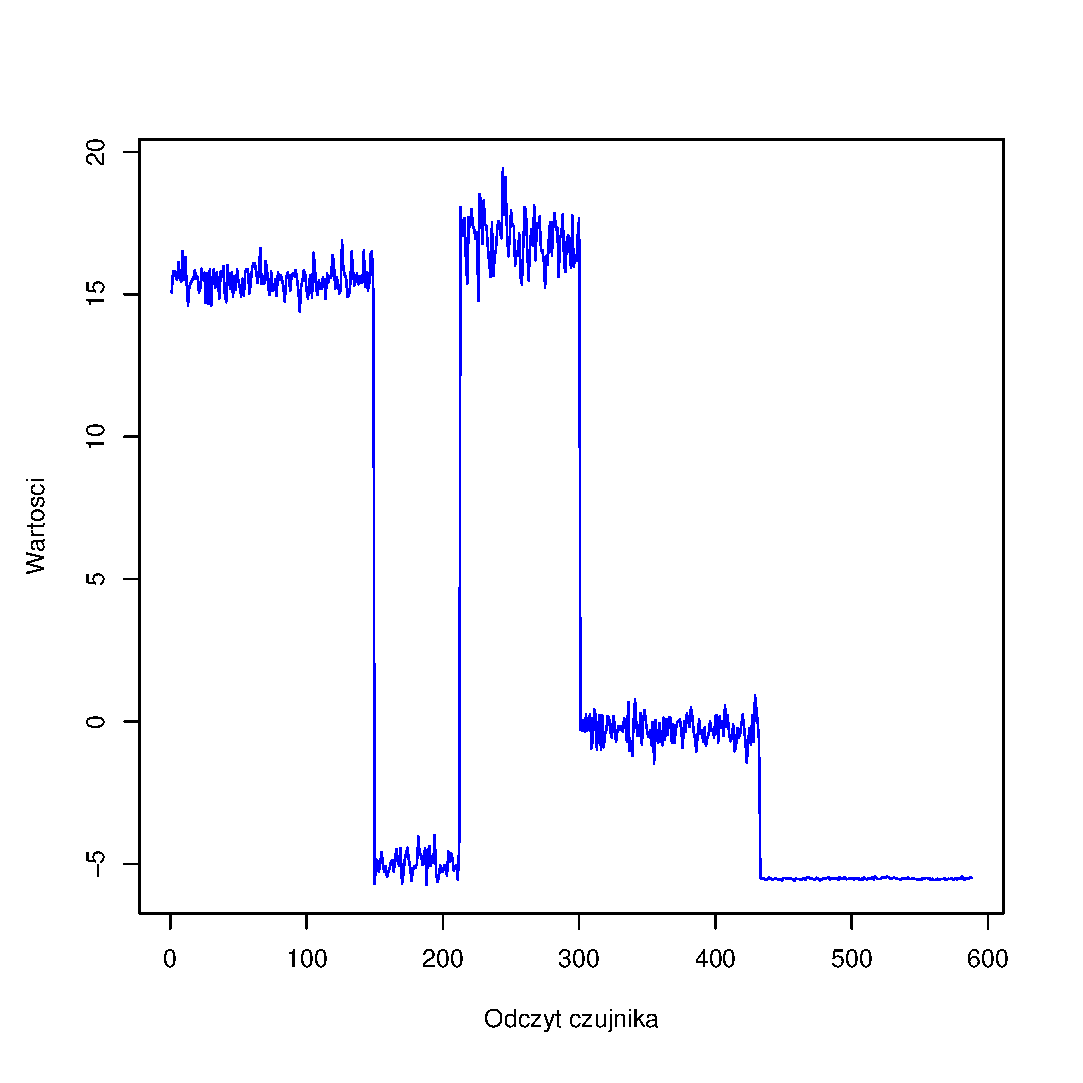
\includegraphics[width=0.6\textwidth]{img/ch-2-data}
	\caption{Zmiana parametrów opisujących strumień danych}
  \label{fig:SignalData}
\end{figure}

% \begin{figure}[htbp]
% \centering
% 	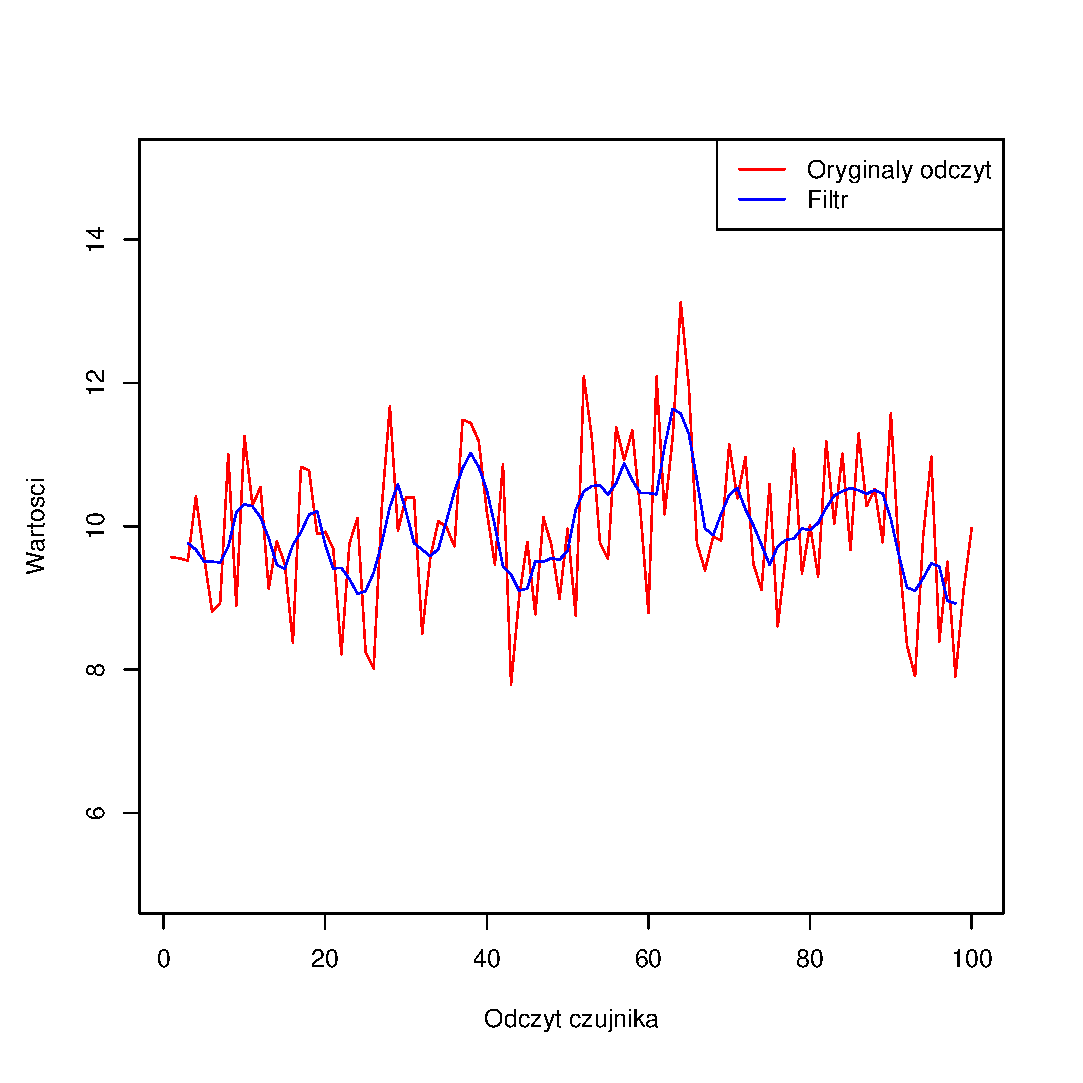
\includegraphics[width=0.5\textwidth]{img/ch-2-filter}
% 	\caption{Procesowanie wsadowe}
%   \label{fig:SignalFilter}
% \end{figure}

\section{Metody wykrywania zmian}

Przez lata z uwagi na swoje znaczenie problem wykrywania zmian skupiał uwagę naukowców i badaczy.
Powstało wiele metod starających się go rozwiązać.
Większość z nich opiera się na:
\begin{itemize}
  \item wartościach progowych,
  \item metodach analitycznych,
  \item analizie skupień (\textit{cluster analysis}),
  \item elementach uczenia maszynowego.
\end{itemize}
W dalszej częsci rozdziału zostaną omówione wartości progowe i metody analityczne
\subsection{Wartości progowe}
Najprostszym sposobem wykrywania sytuacji nietypowych jest ustalenie wartości progowej (\textit{threshold value}),
której przekroczenie oznacza wystąpienie zmiany.
Przykład przedstawiono na rysunku \ref{fig:SignalThreshold}.
Podejście jednak taki wiąże się z pewnymi ograniczeniami.
Dane muszą się charakteryzować względną stabilnością,
tj. powinny mniej więcej utrzymywać się na tym samym poziomie, wzrastać tylko podczas sytuacji nietypowych.
Charakterystyka danych,
także musi być znana,
aby można było dobrać odpowiednią wartość progu.
Strategia skutecznie stosowana w:
\begin{itemize}
  \item systemach awaryjnych,
  \item systamach monitorujących.
\end{itemize}
\begin{figure}[htbp]
\centering
	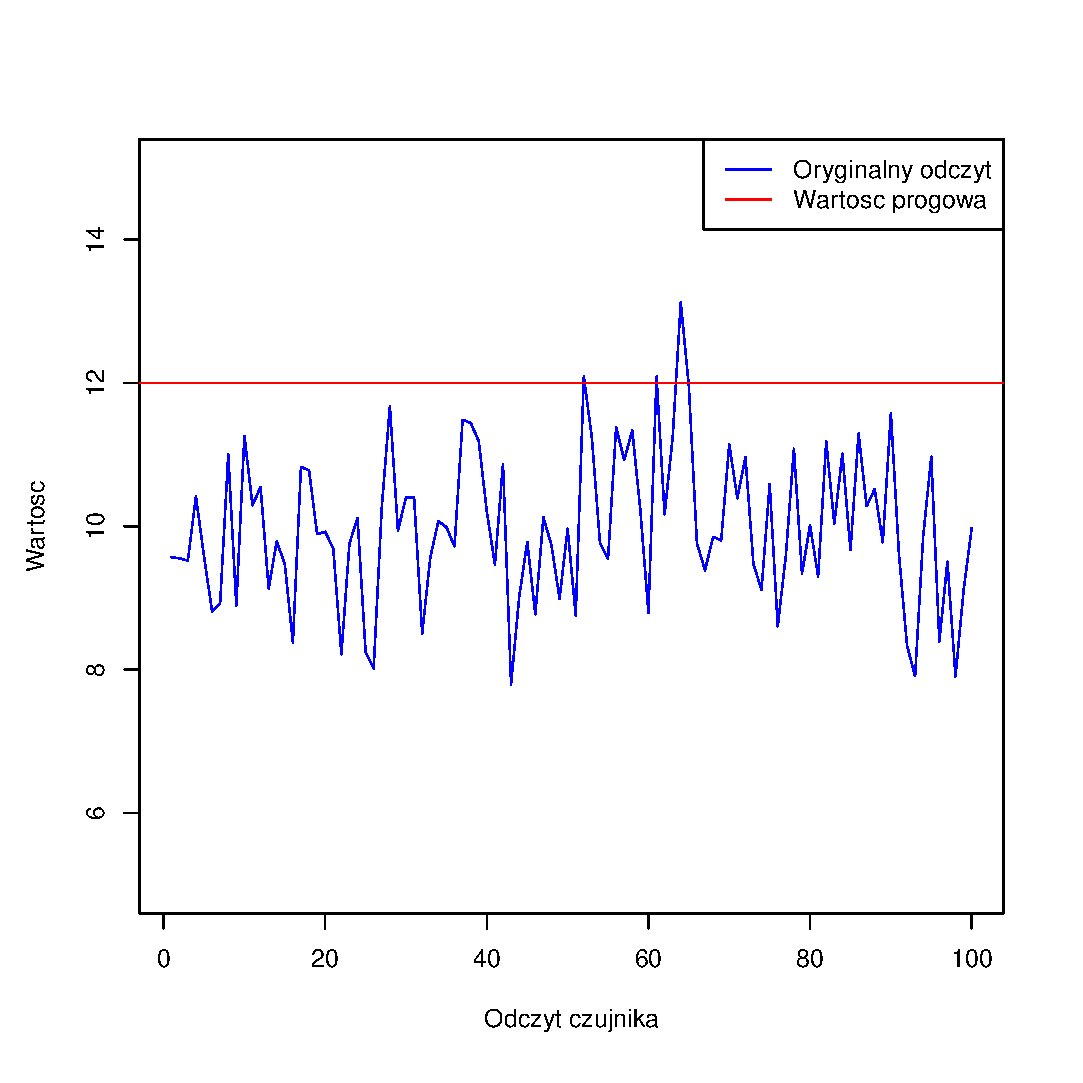
\includegraphics[width=0.6\textwidth]{img/ch-2-threshold}
	\caption{Wykrywanie sytuacji nietypowych -- wartość progowa}
  \label{fig:SignalThreshold}
\end{figure}

\newpage
\subsection{Metody analityczne}

Metody analityczne do rozwiązania problemu wykrywania zmian wykorzystują aparat matematyczny,
głównie statystykę.
Budują na podstawie otrzymywanych danych
oraz wewnętrznego modelu funkcję prawdpobieństwa wystąpienia sytuacji nietypowej.
Na jej podstawie możliwe jest wtedy podjęcie decyzji.
Na rysunku \ref{fig:SignalAnalytics} przedstawiono strumień,
w którym wystąpił szereg zmian.
Poniżej znajduję się odpowiadająca funkcja opisująca prawdopobieństwo wystąpienia zmiany w tym strumieniu.
\begin{figure}[htbp]
\centering
	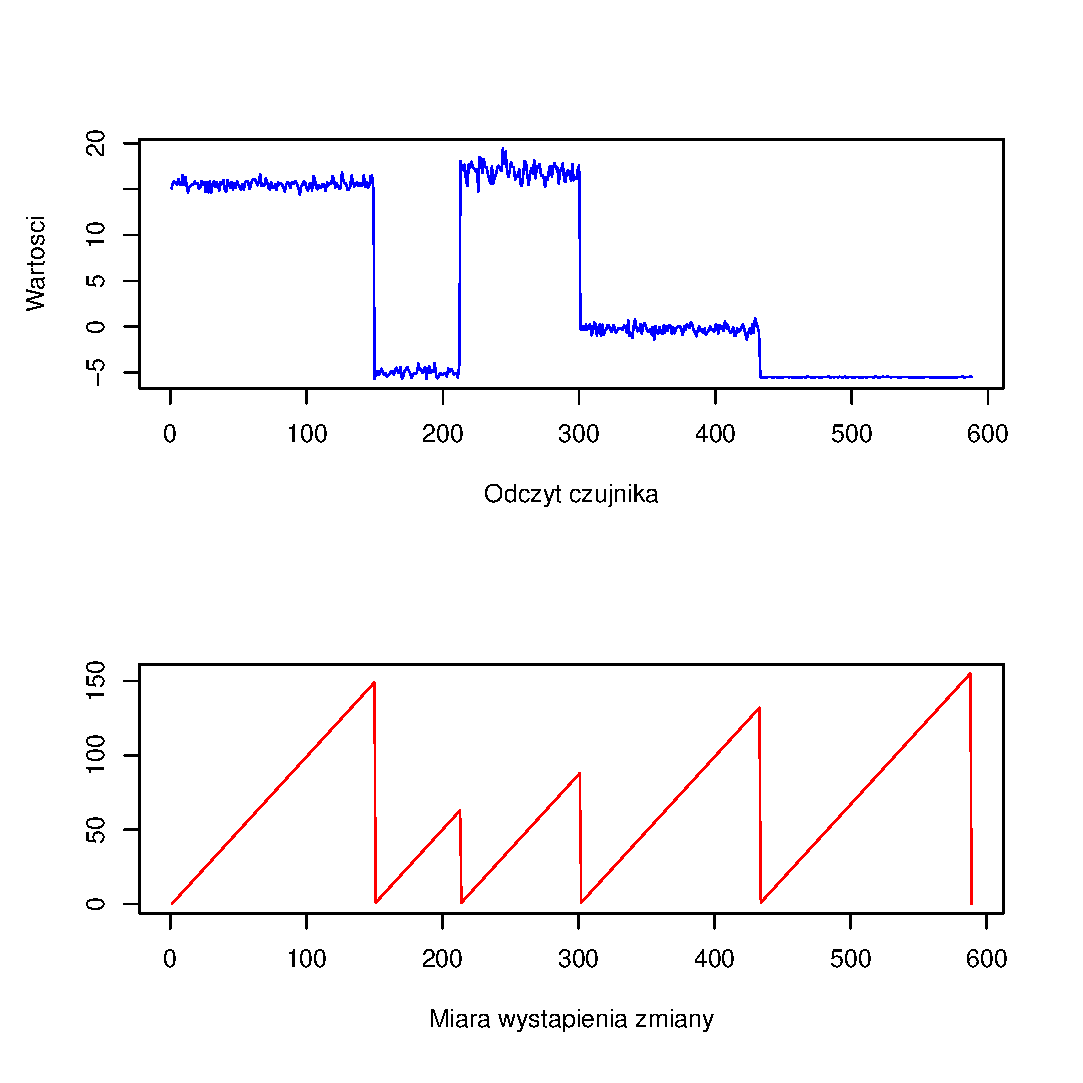
\includegraphics[width=1\textwidth]{img/ch-2-change}
	\caption{Wykrywanie sytuacji nietypowych -- funkcja prawdobieństwa}
  \label{fig:SignalAnalytics}
\end{figure}

Metody analityczne dzielą się na dwie grupy:
\begin{itemize}
  \item \textbf{offline} -- wymagają całego zestawu danych,
  \item \textbf{online} -- przyrostowo analizują dane.
\end{itemize}
Metody offline charakteryzują się większą dokładnością wyników,
za cenę większych opóźnień.
Są wykorzystywane w analizach danych z czujników pogodowych, segmentacji DNA, itp.
Metody online mają praktycznie niezauważalne opóźnienia,
obarczone są jednak większymi błędami.
